% !TEX root = quickstep.tex
\section{Efficient Query Processing} \label{sec:query-opt}
Quickstep builds on a number of existing query processing methods (as described in Section~\ref{overview}). The system also improves on existing methods for specific common query processing patterns. We describe these query processing methods in this section.

Below, we first describe a technique that pushes down certain disjunctive predicates more aggressively than is common in traditional query processing engines. Next, we describe how certain joins can be transformed into cache-efficient semi-joins using \textit{exact filters}. Finally, we describe a technique called \textit{LIP} that uses Bloom filters to speed up the execution of join trees with a star schema pattern.

The unifying theme that underlies these query processing methods is to eliminate redundant computation and materialization using a ``drop early, drop fast'' approach: aggressively pushing down filters in a query plan to drop redundant rows as early as possible, and using efficient mechanisms to pass and apply such filters to drop them as fast as possible.

\subsection{Partial Predicate Push-down}
\label{sec-pushdown-disj-preds}
While query optimizers regularly push conjunctive (\texttt{AND}) predicates down to selections, it is difficult to do so for complex, multi-table predicates involving disjunctions (\texttt{OR}). Quickstep addresses this issue by using an optimization rule that pushes down \textit{partial predicates} that conservatively approximate the result of the original predicate.

Consider a complex disjunctive multi-relation predicate $P$ in the form $P = (p_{1,1} \wedge \dots \wedge p_{1, m_1}) \vee \dots \vee (p_{n,1} \wedge \dots \wedge p_{n, m_n})$, where each term $p_{i,j}$ may itself be a complex predicate but depends only on a single relation. While $P$ itself cannot be pushed down to any of the referenced relations (say $R$), we show how an appropriate relaxation of $P$, $P'(R)$, can indeed be pushed down and applied at a relation $R$.

This predicate approximation technique derives from the insight that if any of the terms $p_{i,j}$ in $P$ does not depend on $R$, it is possible to relax it by replacing it with the tautological predicate $\top$ (i.e., \texttt{TRUE}). Clearly, this technique is only useful if $R$ appears in every conjunctive clause in $P$, since otherwise $P$ relaxes and simplifies to the trivial predicate $\top$. So let us assume without loss of generality that $R$ appears in the first term of every clause, i.e., in each $p_{i,1}$ for $i = 1,2,\ldots,n$. After relaxation, $P$ then simplifies to $P'(R) = p_{1,1} \vee p_{1,2} \vee \ldots \vee p_{1,n}$, which only references the relation $R$.

The predicate $P'$ can now be pushed down to $R$, which often leads to significantly fewer redundant tuples flowing through the rest of the plan. However, since the exact predicate must later be evaluated again, such a partial push down is only useful if the predicate is selective. Quickstep uses a rule-based approach to decide when to push down predicates, but in the future we plan to expand this method to consider a cost-based approach based on estimated cardinalities and selectivities instead.

There is a discussion of join-dependent expression filter pushdown technique in~\cite{BonczNE13}, but the overall algorithm for generalization, and associated details, are not presented. 
The partial predicate push-down can be considered a generalization of such techniques.

Note that the partial predicate push down technique is complimentary to implied predicates used in SQL Server~\cite{sql-server-implied-predicate} and Oracle~\cite{oracle-implied-predicate}.
Implied predicates use statistics from the catalog to add additional filter conditions to the original predicate.
Our technique does not add any new predicates, instead it replaces the predicates from another table to \texttt{TRUE}.

\subsection{Exact Filters: Join to Semi-join Transformation} \label{sec:ef}
A new query processing approach that we introduce (which, to the best of our knowledge, has not been described before) is to identify opportunities when a join can be transformed to a semi-join, and to then use a  fast, cache-efficient semi-join implementation using a succinct bitvector data structure to evaluate the join(s) efficiently. This bitvector data structure is called an \textit{Exact Filter} (EF), and we describe it in more detail below.

To illustrate this technique, consider the SSB~\cite{ssb} query Q4.1 (see Figure~\ref{fig-q41-original}). Notice that in this query the \texttt{part} table does not contribute any attributes to the join result with \texttt{lineorder}, and the primary key constraint guarantees that the \texttt{part} table does not contain duplicates of the join key. Thus, we can transform the \texttt{lineorder} -- \texttt{part} join into a semi-join, as shown in Figure~\ref{fig-q41-semijoin}. During query execution, after the selection predicate is applied on the \texttt{part} table, we insert each resulting value in the join key (\texttt{p\_partkey}) into an \textit{exact filter}. This filter is implemented as a bitvector, with one bit for each potential \texttt{p\_partkey} in the  \texttt{part} table. The size of this bitvector is known during query compilation based on the min-max statistics present in the catalog. (These statistics in the catalog are  kept updated for permanent tables even if the data is modified.) The EF is then probed using the \texttt{lineorder} table. The \texttt{lineorder} -- \texttt{supplier} join also benefits from this optimization.

\begin{figure*}[t]
	\centering
	\begin{subfigure}[bt]{0.3\textwidth}
		\centering
		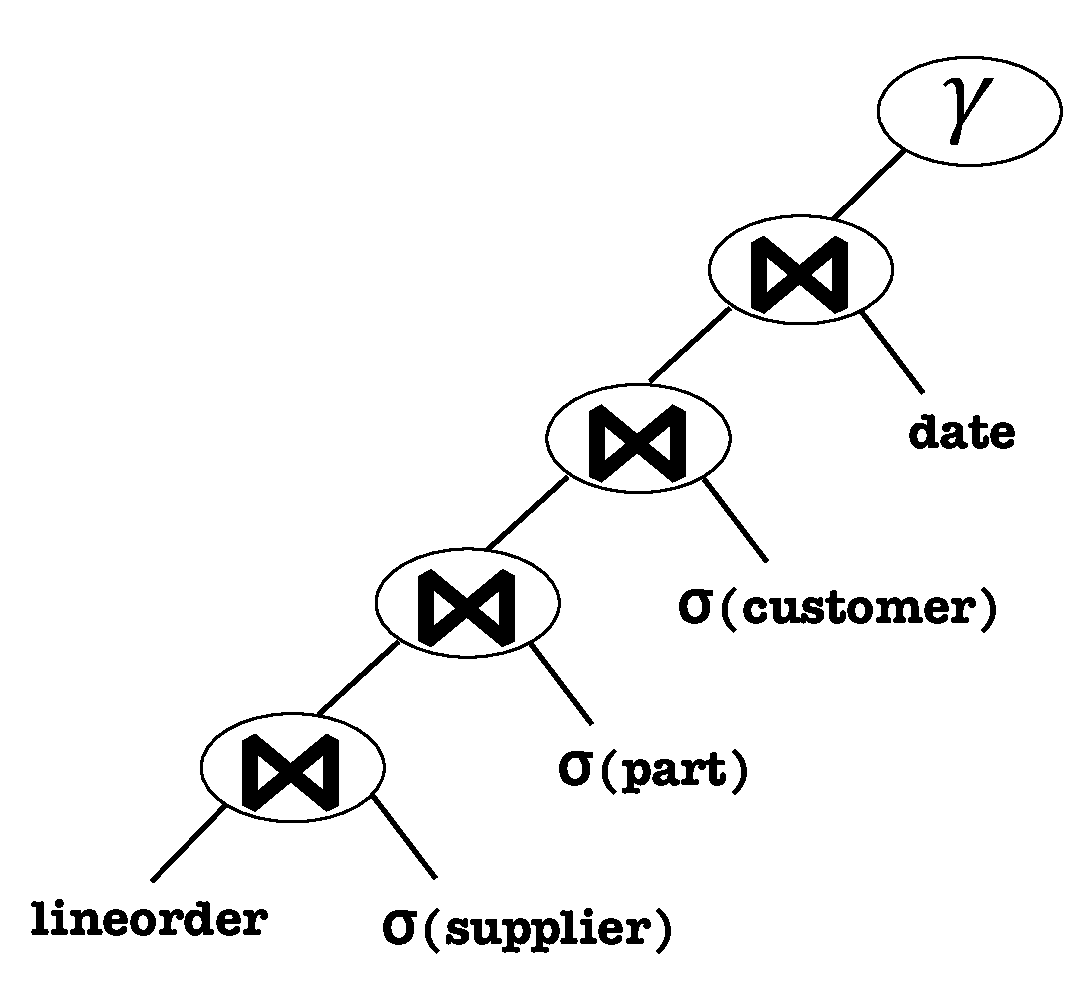
\includegraphics[width=1.0\textwidth,
		height=0.75\textwidth]{system/figures/Q41-original.pdf}
		\caption{Original query plan}
		\label{fig-q41-original}
	\end{subfigure} %
	\begin{subfigure}[bt]{0.3\textwidth}
		\centering
		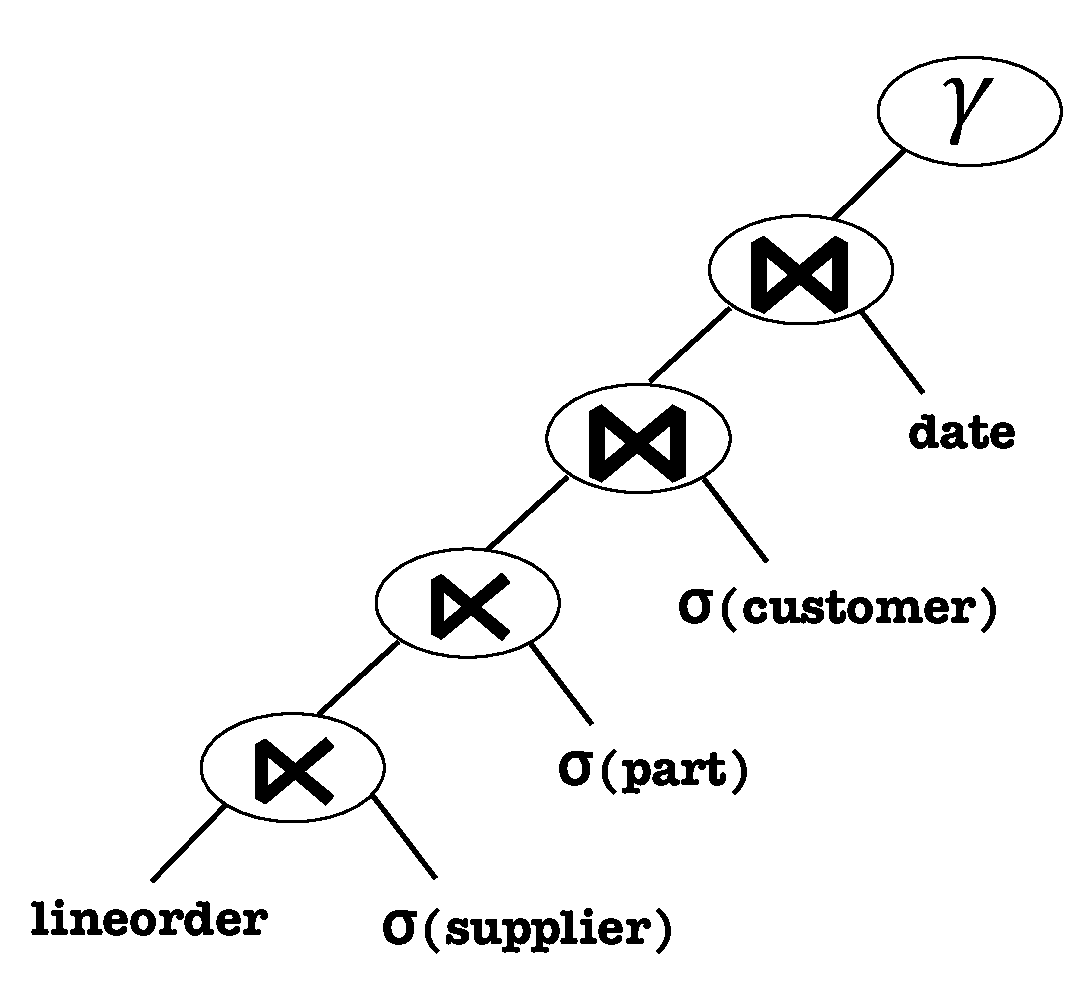
\includegraphics[width=1.0\textwidth,
		height=0.75\textwidth]{system/figures/Q41-semijoin.pdf}
		\caption{Plan using join to semi-join transformation}
		\label{fig-q41-semijoin}
	\end{subfigure} %
	\begin{subfigure}[bt]{0.3\textwidth}
		\centering
		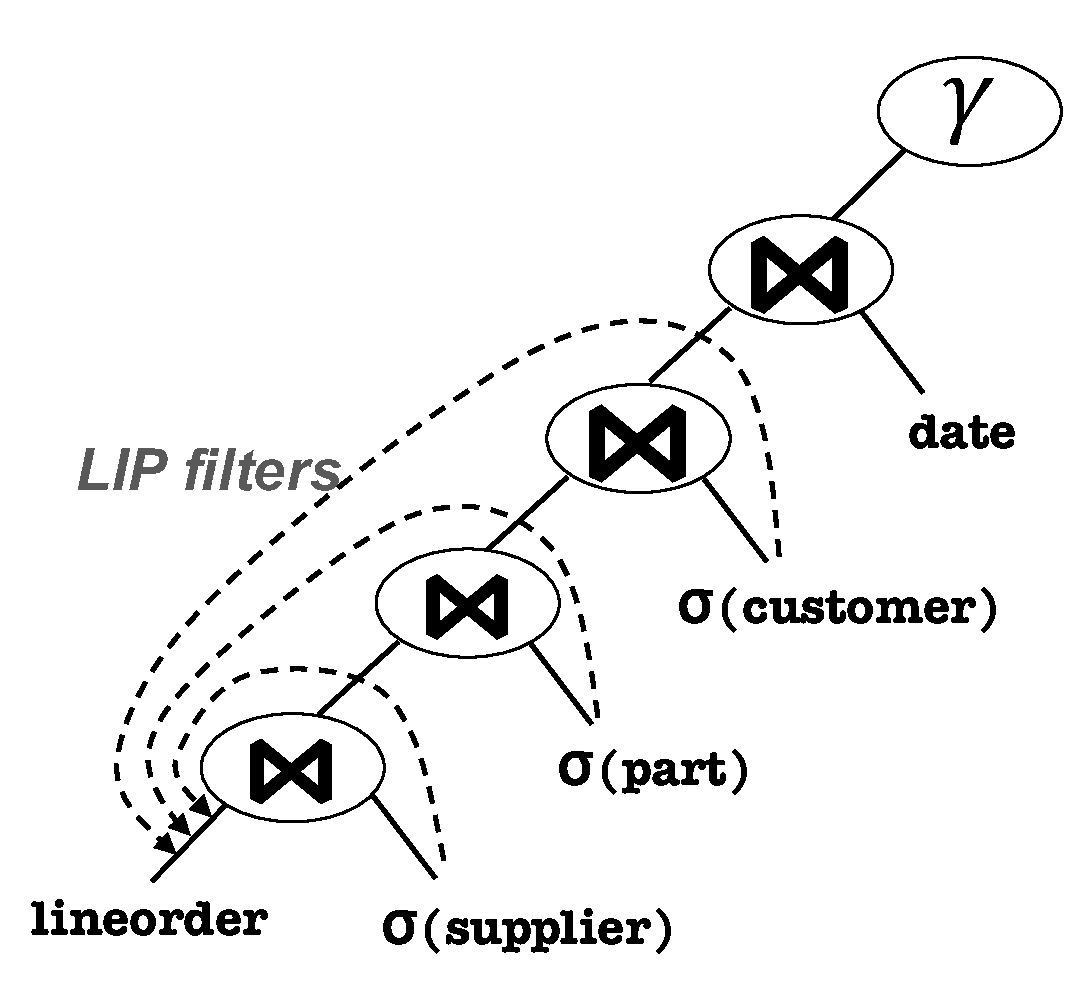
\includegraphics[width=1.0\textwidth,
		height=0.75\textwidth]{system/figures/Q41-LIP.pdf}
		\caption{Query plan using LIP (only)}
		\label{fig-q41-lip}
	\end{subfigure} %
	\caption{\textbf{Query plan variations for SSB Query 4.1}}
\end{figure*}

The implementation of semi-join operation using EF rather than hash tables improves performance for many reasons. First, by turning insertions and probes into fast bit operations, it eliminates the costs of hashing keys and chasing collision chains in a hash table. Second, since the filter is far more succinct than a hash table, it improves the cache hit ratio. Finally, the predictable size of the filter eliminates costly hash table resize operations that occur when selectivity estimates are poor.

The same optimization rule also transforms anti-joins into semi-anti-joins, which are implemented similarly using EFs.

\subsection{Lookahead Information Passing (LIP)} \label{sec:lip}
Quickstep also employs a join processing technique called LIP that combines the ``drop early'' and ``drop fast'' principles underlying the techniques we described above. We only briefly discuss this technique here, and refer the reader to related work~\cite{DBLP:journals/pvldb/ZhuPSP17} for more details.

Consider SSB Query 4.1 from Figure~\ref{fig-q41-original} again. The running time for this query plan is dominated by the cost of processing the tree of joins. We observe that a \texttt{lineorder} row may pass the joins with \texttt{supplier} and \texttt{part}, only to be dropped by the join with \texttt{customer}. Even if we assume that the joins are performed in the optimal order, the original query plan performs redundant hash table probes and materializations for this row. The essence of the LIP technique is to look ahead in the query plan and drop such rows early. In order to do so efficiently, we use \emph{LIP filters}, typically an appropriately-configured Bloom filter~\cite{Bloom70Space}.

The LIP technique is based on semi-join processing and sideways information passing~\cite{Bernstein1981SemiJoin, Ives2008Sideways, Beeri1987Magic}, but is applied more aggressively and optimized for left-deep hash join trees in the main-memory context. For each join in the join tree, during the hash-table build phase, we insert the build-side join keys into an LIP filter. Then, these filters are all passed to the probe-side table, as shown in Figure~\ref{fig-q41-lip}. During the probe phase of the hash join, the probe-side join keys are looked up in all the LIP filters prior to probing the hash tables. Due to the succinct nature of the Bloom filters, this LIP filter probe phase is more efficient than hash table probes, while allowing us to drop most of the redundant rows early, % in the join tree,
effectively pushing down all build-side predicates to the probe-side table scan.

During query optimization, Quickstep first pushes down predicates (including partial push-down described above) and transforms joins to semi-joins. The LIP technique is then used to speed up the remaining joins. Note that our implementation of LIP generalizes beyond the discussion here to also push down filters across other types of joins, as well as aggregations. In addition to its performance benefits, LIP also provably improves robustness to join order selection through the use of an adaptive technique, as discussed in detail in~\cite{DBLP:journals/pvldb/ZhuPSP17}.

